
\chapter{Conclusion and Perspectives}\label{chap:conclusion}
\markright{{~{\rm \ref{chap:conclusion}}. Conclusion and Perspectives}\hfill}{}


\vspace*{\fill}

In this last chapter we detail the different contributions contained within this  thesis and we point out possible extension that can be considered in the future. The proposed methods span all the different contributions of this thesis. We also enumerate the software packages that have been developed. 

\vspace{10pt}
\minitoc

\vspace*{\fill}


\newpage

\section{Contributions}

In this thesis we have examined several aspects of the pipeline through which an fMRI datasets can be analyzed. We have made contributions at different stages of this pipeline.

In Chapter~\ref{chap:hrf_estimation} we have studied a problem of \emph{feature extraction}. The goal of this feature extraction step is to output \mbox{time-independent} activation maps from the BOLD time series. In this context we have introduced a new model for the joint estimation of hemodynamic response function (HRF) and brain activation coefficient. 
The novelty of our method stems from the observation that the formulation of the GLM model with a common (but unknown) HRF across conditions translates into a rank constraint on the vector of estimates. This allows to specify the model as a smooth optimization problem and to use gradient-based methods for its estimation.


A popular application of supervised learning to reveal cognitive mechanisms in fMRI studies is the problem of \emph{brain decoding}, in which the goal is to predict some information about the stimuli given the activation coefficients. In Chapter~\ref{chap:decoding_ordinal} we examine the setting of practical importance in which the target variable consist of discretely ordered values. We identified two loss functions that are appropriate for the task: the absolute error and the pairwise disagreement. We presented several models based on the minimization of a convex surrogate of these loss functions. We examined their performance on both synthetic and two real world fMRI datasets.


Motivated by its applicability to decoding studies we turned in Chapter~\ref{chap:consistency} to study some theoretical properties of \emph{ordinal regression} models. We provided an analysis of the Fisher consistency properties of a rich family of surrogate loss functions, including proportional odds and support vector ordinal regression. For all the surrogates considered, we either proved consistency or provided sufficient conditions under which these approaches are consistent. 


\section{Research Perspectives}



% \begin{figure}
% 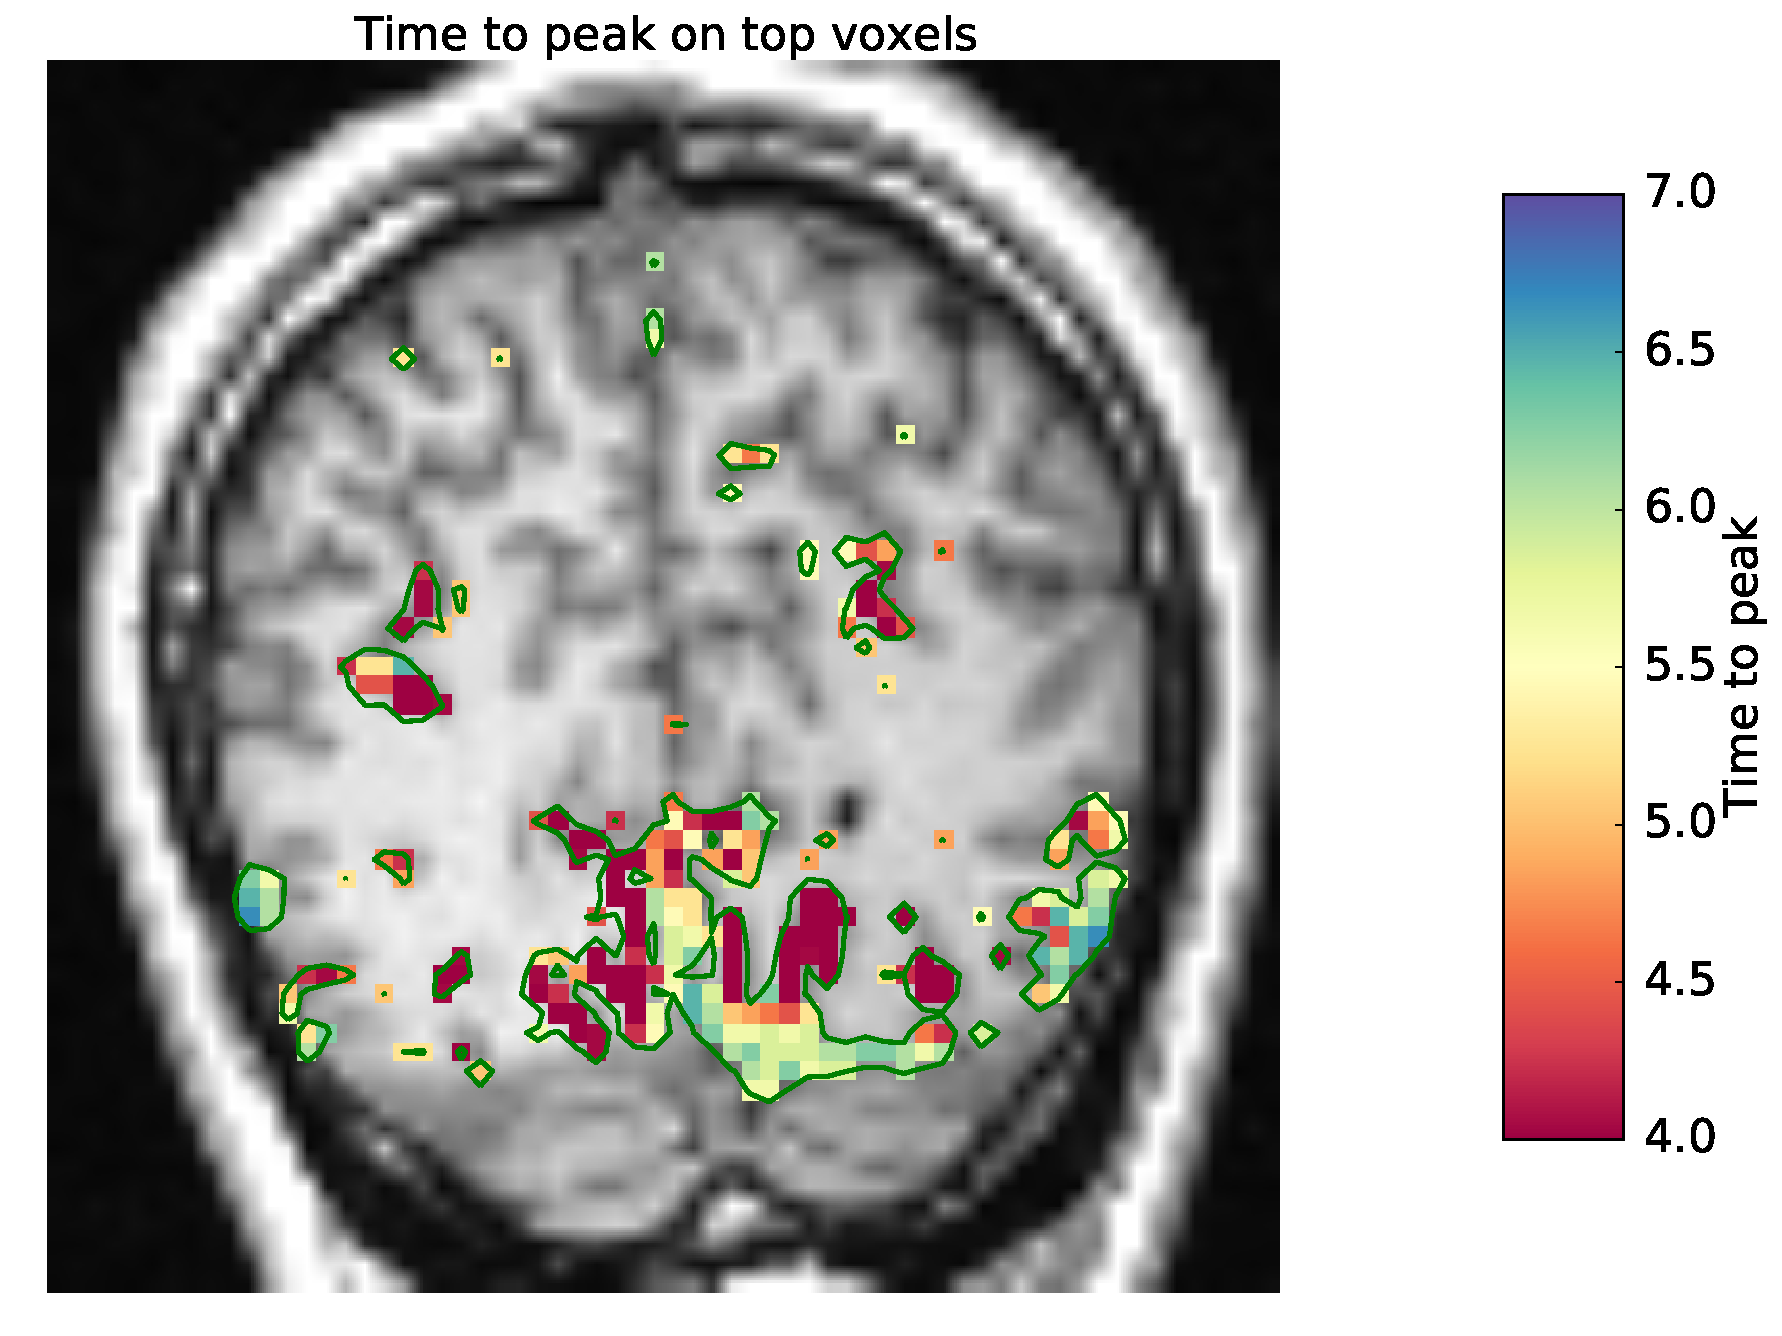
\includegraphics[width=\linewidth]{chapter_3/brain_ttp.pdf}
% \caption{ }
% \end{figure}

\subsection{A tensor formulation of R1-GLM}

Although the R1-GLM model presented in Chapter~\ref{chap:hrf_estimation} has faster execution times than methods that implement similar assumptions~\citep{Makni2008,vincent2010spatially,Degras2014}), the algorithm still does not use all the structure within the problem. 

For example, the algorithm fits independently a R1-GLM on every voxel (for around $5 \times 10^4$ voxels in a fMRI volume) without taking into account that \emph{the design matrix is the same for all voxels}. In this context, a possible line of research is to use a \emph{tensor-based formulation} of the R1-GLM model to incorporate this structure within the solver. 



\begin{figure}
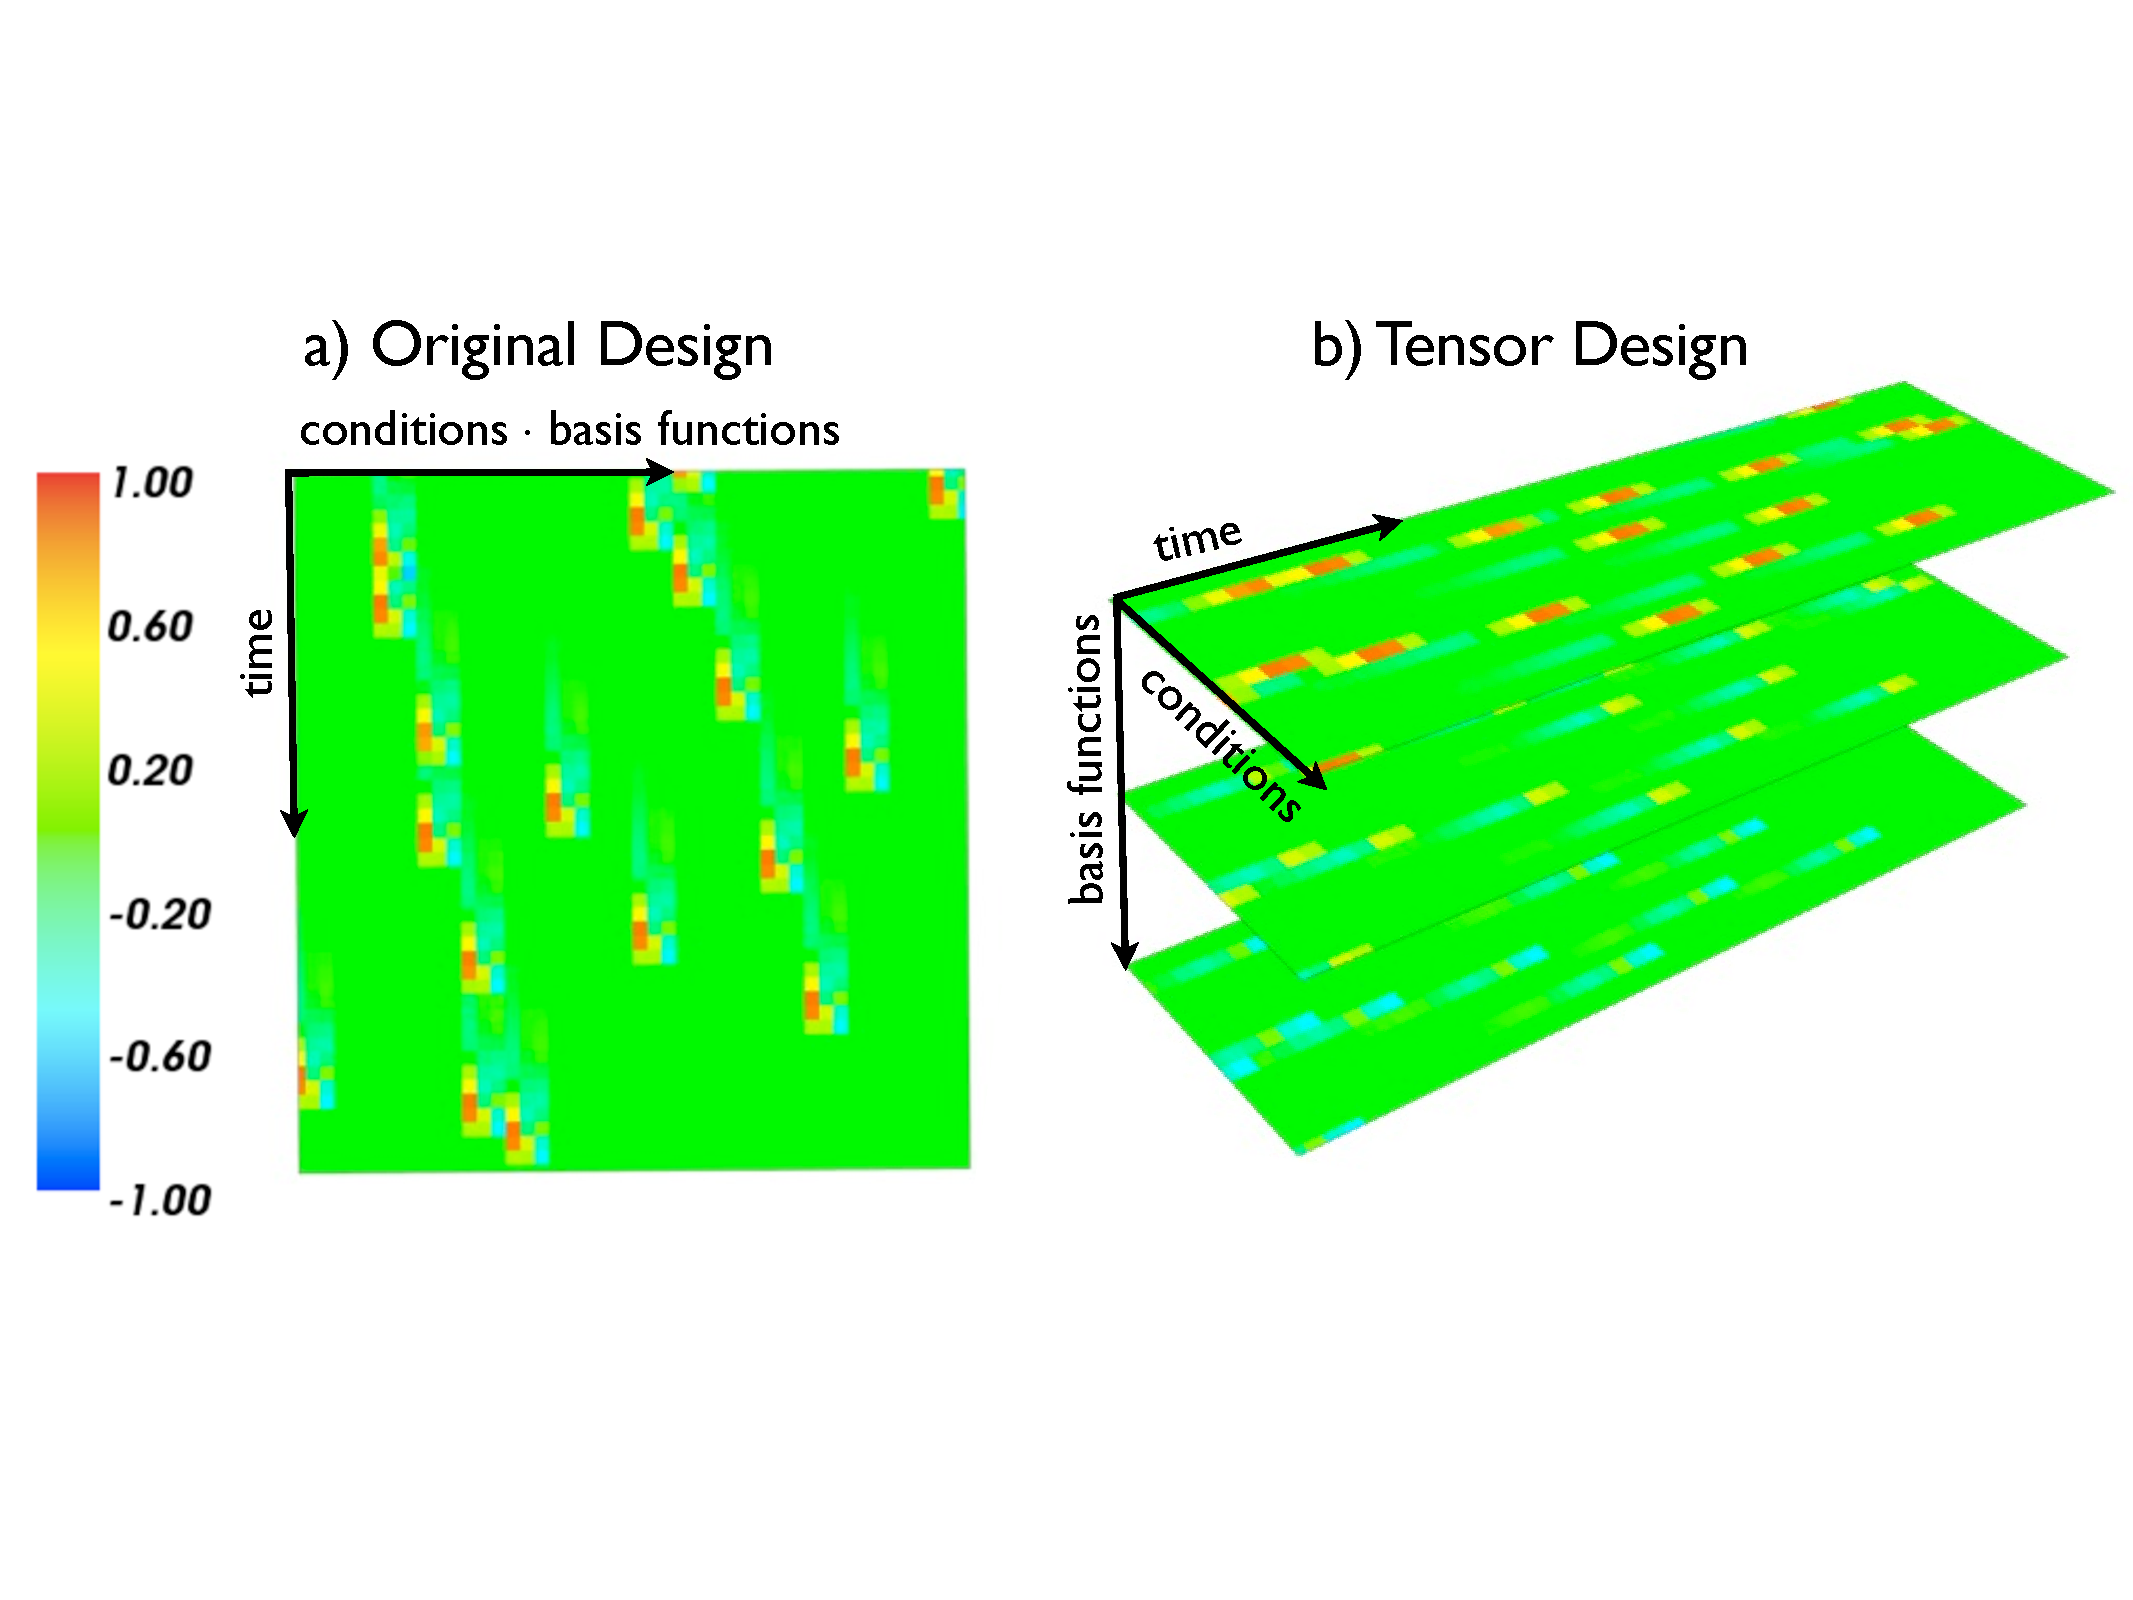
\includegraphics[width=\linewidth]{chapter_6/matrix_vs_tensor_glm.pdf}
\end{figure}

Let $\B{X} \in \RR^{n \times k d}$ be the design matrix of the \gls{GLM}. This matrix can be naturally represented as the tensor $\mathcal{X} \in \RR^{n \times k \times d}$ that verifies that its matrizialization along the last axis corresponds to the design matrix $\B{X}$. In this case, using the $n$-mode tensor product~\citep{Kolda2009} we have the identity
$
\B{X}\text{vec}(\B{h}\bfbeta^T) = \mathcal{X} \times_2 \B{h} \times_3 \bfbeta
$,
hence the R1-GLM can be seen as the minimization of the objective function
$$\|\B{y} - \mathcal{X} \times_2 \B{h} \times_3 \bfbeta\|^2$$
subject to the usual constraints on $\B{h}, \bfbeta$. Due to its analogies with a linear least squares problem, it seems reasonable to think that a tensor factorization of $\mathcal{X}$ (such as CP/PARAFAC or Tucker) might be able to solve or accelerate the optimization of this model.

\subsection{Uniqueness of solution for R1-GLM}

The R1-GLM model, being non-convex, comes with no guarantees of convergence to a global optimum for the algorithms considered.

However, some scarce theoretical results exist. For the case of infinite data (which would correspond in our model to an infinite number of fMRI scans), the uniqueness of solution of a similar model was proved by~\citep{bai2006least}. A possible area of research is to extend these results to the more practical setting of a limited number of samples.



\subsection{Parcel R1-GLM model}


This is a different extension of the R1-GLM model presented in Chapter~\ref{chap:hrf_estimation} that aims at reducing the amount of HRFs estimated within the model.

Within the context of HRF estimation, some studies have proposed to perform the estimation of an HRF in a set of neighboring voxels called a \emph{parcel}, thus taking advantage of the spatially dependent nature of
fMRI~\citep{Wang2013,Chaari2012,Badillo2013a}. 

The notion of parcel, i.e., a brain region which shares the same HRF, can be trivially incorporated into the R1-GLM model, and results in a modified R1-GLM model. Given $m$ voxels in the parcel, let $\B{y} = [\mathbf{y}_1, \B{y}_2, \ldots, \B{y}_m]$ the concatenation of the BOLD signal for the voxels within the parcel and let $\B{X}$ be the matrix formed by a block-diagonal matrix with $m$ blocks in which every block is the design matrix for the current experiment. Then the R1-GLM model that assumes the HRF constant across the parcel can be written as
\begin{eqnarray}
\begin{aligned}
\hat{\B{h}}, ~\hat{\bfbeta},~ \hat{\bfomega} ~=~& \argmin_{\B{h}, \bfbeta, {\bfomega}} ~ \frac{1}{2}\|\B{y} - \mathbf{X} \vecop(\B{h} \bfbeta) - \B{Z} {\bfomega}\| ^2\\
&\text{subject to } \|\B{B} \B{h}\|_{\infty} = 1 \text{ and } \langle \B{B} \B{h}, \B{h}_{\text{ref}}\rangle > 0 \enspace ,
\end{aligned}
\end{eqnarray}
where $\bfbeta = [\bfbeta_1, \ldots, \bfbeta_m]$ contains the activation coefficients for the different voxels within the region. Phrased differently, the estimation of a R1-GLM model within a parcel is itself a R1-GLM model with a modified design matrix.

However, these approaches must face the problem of choosing the right brain parcellation. 
An interesting approach, named
\mbox{hemodynamically-informed}
parcellations~\citep{Chaari2012,Badillo2013a} relies on the computation of 
a large number of estimations at the voxel or \mbox{sub-parcel} level.



% There is empirical evidence that constraining further the HRF to be the same on a parzel helps with the identification. 

% But now you have to decide how to choose the parzel. The best choice of parzels for estimating the HRF is an open problem.

% One of the most interesting parameters of the HRF is the time to peak. Examining the TTP of the best-estimated voxels on the Kay dataset.


\subsection{Weaker conditions for the consistency of threshold-based ordinal regression methods}

In Chapter~\ref{chap:consistency} we have presented consistency results for some ordinal regression methods. For threshold-based methods, in the practical setting in which the thresholds are constant across samples (a setting that we called model with \emph{threshold-based decision function}), we have only been able to prove consistency under very restrictive conditions on the underlying probability distribution.

It is possible that similar consistency results can be obtained with weaker conditions on the probability distribution, which would result in conditions that are widely applicable. For example, in~\citep[Section 2]{Herbrich1999}, the authors present the cumulative models of~\citep{McCullagh1980} (described in Section~\ref{sec:problem_setting}) as a consequence of a stochastic ordering in the sample space. 

The stochastic ordering assumption can be described as follows. Given the sample space $\mathcal{X}$ and a target space $\mathcal{Y}$, then for all different $x_1, x_2 \in \mathcal{X}$ either
$$
P(y \leq r | X=x_1) \geq P(y \leq r | X=x_2) \text{ for all } r \in \mathcal{Y}
$$
or
$$
P(y \leq r | X=x_1) \leq P(y \leq r | X=x_2) \text{ for all } r \in \mathcal{Y}
$$

The authors then conclude that stochastic ordering is satisfied by a model of the form
$$
g^{-1}(P(y \leq r|X=x)) = \theta_r - f(x)
$$
hence it seems reasonable to think that a stochastic ordering could be a sufficient condition in order to obtain consistency -- at least for the cumulative logit model. 


% Stochastic ordering~\citep{bauerle2006stochastic, el2013empirical} can be a first line of investigation since it has already been used to describe the assumptions behind ordinal regression.





\subsection{Application of ordinal regression methods to multiclass classification }

Although ordinal regression methods have been initially developed for loss functions that minimize a distance between the labels, our theoretical results show that some ordinal regression methods are instead consistent to the 0-1 loss\sidenote{We recall that (although in a degenerate sense), the 0-1 loss does verify the V-shape property.}, i.e., with the usual loss used in multiclass classification. This suggests that some ordinal regression methods might be competitive in the context of multiclass classification. One of the advantages of ordinal regression models is that for linear decision functions, the learning only requires the estimation of $p + k - 1$ parameters versus e.g. $p\times (k-1)$ in the case of one-vs-all multiclass classification, where $p$ is the dimensionality of the dataset and $k$ is the number of classes. It is possible that these methods have applications for the estimation of multiclass classification rules in very high-dimensional settings, although its usefulness still needs to be determined.


\newpage



\vspace*{\fill}
\section{Publications by the author}
\begin{fullwidth}
{\center

% This thesis contains material contained in the following publications.

\vspace{0pt}{\bf \color{msblue} \textsc{chapter III}}

\begin{itemize}
\item V. Borghesani, {\bf F. Pedregosa}, E. Eger, M. Buiatti, and M. Piazza, \emph{“A perceptual-to-conceptual gradient of word coding along the ventral path”} Proceedings of the 4th International Workshop on Pattern Recognition in Neuroimaging, 2014.
\end{itemize}

\vspace{10pt}
{\bf \color{msblue} \textsc{chapter IV}}
\begin{itemize}
\item {\bf F. Pedregosa}, M. Eickenberg, P. Ciuciu, B. Thirion, and A. Gramfort \emph{``Data-driven HRF estimation for encoding and decoding models''} NeuroImage, Volume 104, 1 January 2015, Pages 209-220.

\item {\bf F. Pedregosa}, M. Eickenberg, B. Thirion, and A. Gramfort, \emph{“HRF estimation improves sensitivity of fMRI encoding and decoding models”} Proc. 3nd Int. Work. Pattern Recognit. NeuroImaging, 2013.
\end{itemize}

\vspace{10pt}
{\bf \color{msblue} \textsc{chapter V}}
\begin{itemize}
\item {\bf F. Pedregosa}, E. Cauvet, G. Varoquaux, C. Pallier, B. Thirion, and A. Gramfort, \emph{``Learning to rank from medical imaging data''}, in Proceedings of the 3rd International Workshop on Machine Learning in Medical Imaging, 2012.
\item {\bf F. Pedregosa}, E. Cauvet, G. Varoquaux, C. Pallier, B. Thirion, and A. Gramfort, \emph{``Improved brain pattern recovery through ranking approaches''}. 2nd International Workshop on Pattern Recognition in NeuroImaging, Jul 2012
\item Y. Bekhti, N. Zilber, {\bf F. Pedregosa}, P. Ciuciu, V. Van Wassenhove, and A. Gramfort, \emph{``Decoding perceptual thresholds from MEG/EEG''}. Pattern Recoginition in Neuroimaging (PRNI) (2014)
\end{itemize}

\vspace{10pt}
{\bf \color{msblue} \textsc{chapter VI}}
\begin{itemize}
\item {\bf F. Pedregosa}, F. Bach, and A. Gramfort, \emph{``On the Consistency of Ordinal Regression Methods''}.
\end{itemize}

\vspace{10pt}
{\bf \color{msblue} \textsc{other publications}}
\begin{itemize}
\item L. Buitinck, G. Louppe, M. Blondel, {\bf F. Pedregosa}, A. Mueller, et al.. \emph{``API design for machine learning software: experiences from the scikit-learn project''}. European Conference on Machine Learning and Principles and Practices of Knowledge Discovery in Databases, 2013.

\item M. Eickenberg, {\bf F. Pedregosa}, S. Mehdi, A. Gramfort, B. Thirion. \emph{``Second order scattering descriptors predict fMRI activity due to visual textures''}. 3rd International Workshop on Pattern Recognition in NeuroImaging, 2013. 

\item A. Abraham, {\bf F. Pedregosa}, M. Eickenberg, P. Gervais, A. Mueller, J. Kossaifi,  B. Thirion and G. Varoquaux (2014). \emph{``Machine learning for neuroimaging with scikit-learn''}. Frontiers in neuroinformatics, 8.

\item F. Yepes-Calderon, {\bf F. Pedregosa}, F., Thirion, B., Wang, Y., and Lepore, N. (2014, March). Automatic pathology classification using a single feature machine learning support-vector machines. In SPIE Medical Imaging (pp. 903524-903524). International Society for Optics and Photonics.
\end{itemize}
}
\end{fullwidth}
\vspace*{\fill}


\newpage

\section{Software}

A number of software distributions have been developed within the context of this thesis.

\subsection{hrf\_estimation}\label{subsec:hrf_estimation}

This package implements method for the joint estimation of hemodynamic response function (HRF) and activation coefficients (aka beta-maps) from fMRI data presented in Chapter~\ref{chap:hrf_estimation}. Full documentation for this package, including an example IPython notebook can be found at 

\vspace{15pt}
\centerline{ \url{http://pythonhosted.org/hrf_estimation/}}

\subsection{mord}

Ordinal Regression algorithms. Module that implements the ordinal regression models used in Chapter~\ref{chap:decoding_ordinal}. The code can be found at the URL

\vspace{15pt}
\centerline{ \url{https://github.com/fabianp/mord}}

\subsection{pysofia}~\label{subsec:pysofia}

PySofia is a python wrapper around the methods present in the C++ sofia-ml library. These include Stochastic Gradient Descent implementations of some ranking algorithms, notably RankSVM~\citep{sculley2009large}.

\vspace{15pt}
\centerline{\url{https://pypi.python.org/pypi/pysofia/}}

\subsection{memory\_profiler}

\begin{marginfigure}
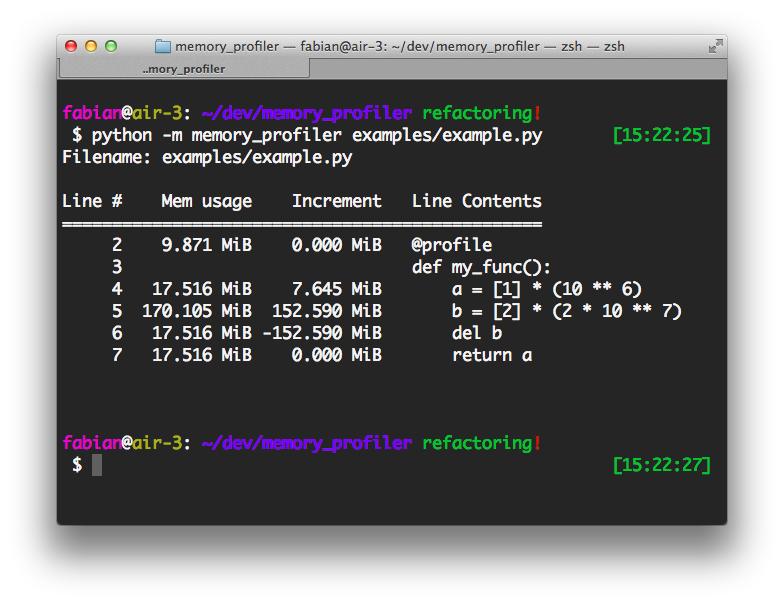
\includegraphics[width=1.2\linewidth]{chapter_6/memory_profiler_screenshot.png}
\vspace{-10pt}\caption{The memory\_profiler module allows to quickly analyze the memory consumption of a program by using the line-by-line profiling (in the picture) or the time-based memory profiling.}
\end{marginfigure}

This is a python module for monitoring memory consumption of a process as well as line-by-line analysis of memory consumption for python programs. It is a pure python module.

\vspace{15pt}
\centerline{\url{https://pypi.python.org/pypi/memory_profiler}}
\vspace{10pt}



The presentation of this module won the \emph{Best Poster Award} at the conference EuroScipy 2012 (European Scientific Computing in Python)


\newpage

\begin{fullwidth}
\bibliographystyle{plainnat}
\bibliography{chapter_6/biblio6}
\end{fullwidth}
